%%%%%%%%%%%%%%%%%%%%%%%%%%%%%%%%%%%%%%%%%%%%%%%%%%%%%%%%%%%%%%%%%%%%%%%%%%%
\chapter{Introduction}
%%%%%%%%%%%%%%%%%%%%%%%%%%%%%%%%%%%%%%%%%%%%%%%%%%%%%%%%%%%%%%%%%%%%%%%%%%%

Pathfinding algorithms are methods of finding a path between two vertices in  
a graph. Most pathfinding problems are concerned with finding the shortest
path between two vertices, if there is more than one possible path. There had 
been many pathfinding algorithms that had been developed throughout the years 
such as Minimum Spanning Tree (MST), Prim's Algorithm\cite{Prim1957}, and the A*
algorithm, which will be used in this paper.\cite{HartNilssonRaphael1968}

Functional programming is one of the major programming paradigms where computations 
are done by function composition. Along with this, purely-functional programming is 
a subparadigm of functional programming where there are no side-effects (e.g, variable mutability).
One of the major challenges of parallel programming is controlling the order of execution
to prevent \emph{race conditions}, which can often lead to bugs and are hard to maintain.
However, since purely-functional programming languages such as Haskell\cite{HaskellSite}
have no mutability and computations lead to the same result regardless of the order, they 
are a perfect candidate for writing parallel programs.\cite{Hammond2011} 
This research aims to find a parallel implementation of the existing A* pathfinding algorithm
using a purely-functional setting with attention to program performance in terms of time and space 
complexity. \cite{ZaghloulAlJami2017, WeinstockHolladay}
In turn, this helps in the advancement of different programming languages that feature 
functional programming and lambda expressions when it comes to purely-functional algorithms and data structures.

% Likewise, pure functions can be reasoned easier than functions with side-effects.
% Importing pure functions into other languages that can be used as proof assistants 
% such as Coq or Agda\cite{Breitner2018, SpectorZabusky2018, ElBakouny2017} is possible 
% and gives a better assurance of a bug-free parallel system.



% The Shortest Common Superstring (SCS) problem, known to be NP-Complete,
% seeks the shortest string that contains all strings from a given set.
% In this paper, we provide the summary of the problem and some of its characteristics.

% The SCS problem has been extensively studied for its
% applications in string compression and DNA sequence assembly \cite{Ma2009}.

% The superstring problem has applications to data storage,
%  specifically, data (string) compression \cite{Gallant1980}. 
% In many programming languages, a character string may be 
% represented by a pointer to that string. 
% The problem for the compiler is to arrange strings 
% so that they may be ``overlapped'' as much as possible.

% DNA sequence assembly is another  problem to which an SCS algorithm is known to apply.
% The $sequencing$ problem in molecular biology is to ``read'' a string of DNA,
% which can be viewed as a string over the alphabet \{A,C,G,T\}. Sequencing produces such a large number of fragments that
% almost all genome positions are covered by many fragments. This short fragments
% thus have large overlaps between other pieces. Hence, they can be given as an input to SCS algorithm.
% Figure \ref{fig:dna-overlap} shows an overlap graph consisting DNA reads (or fragments) as nodes. 



% \begin{figure*}
% \centering
% \fbox{
% \scalebox{0.65}{
% 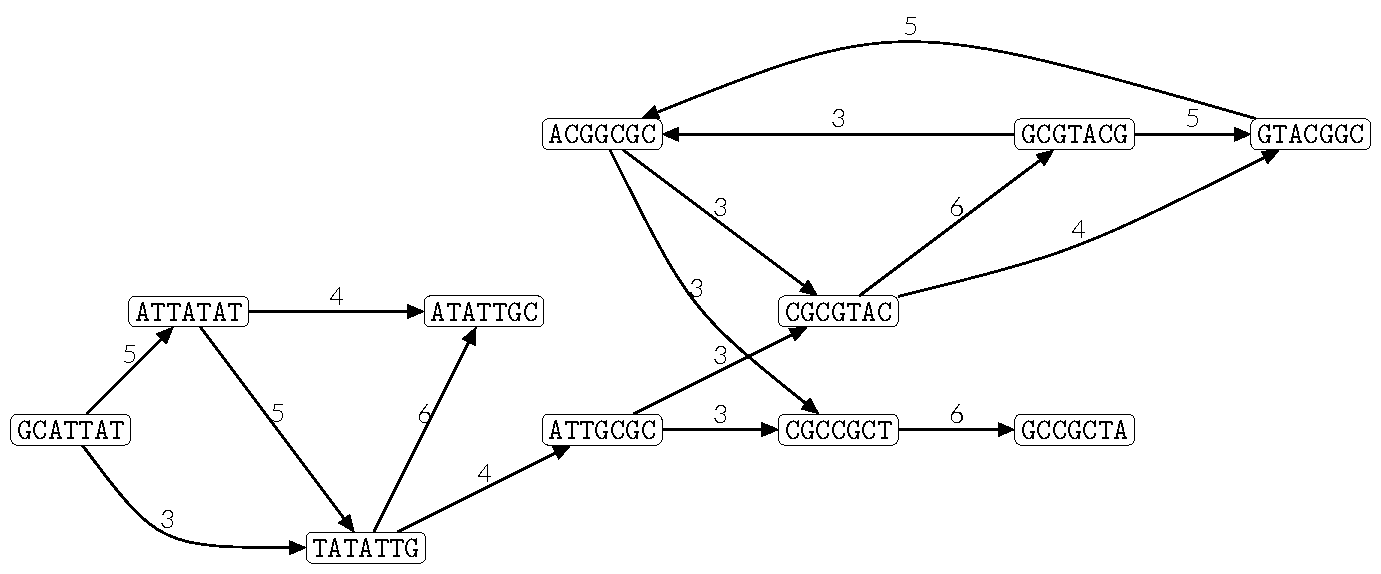
\includegraphics{fig-overlaps-dns-example}
% }}
% \caption{Sample overlap graph with each adjacent nodes 
% having at least $k = 3$ overlaps. The original string is \texttt{GCATTATATATTGCGCGTACGGCGCCGCTACA}.}
% \label{fig:dna-overlap}
% \end{figure*}	

% In \cite{Ma2009}'s paper, SCS was used to analyze DNA sequence assembly using
% a greedy algorithm. 

\section{Project Context}
The A* pathfinding algorithm is mostly used as a pathfinding algorithm
for video games. While most games are written in an imperative and 
object-oriented language such as C\#, C++, and JavaScript, it is 
possible to write video games in a functional languages
using a reactive functional programming approach.\cite{Cheong2006}
Though, functional programming had been getting more popular recently, imperative programming 
still dominates the industry, thus more algorithms are designed with imperative programs in mind.\cite{CLRS,Skiena,Knuth1997}
Thus, the need for functional approaches to familiar algorithms should be addressed in order 
for functional programming to be used more widely in video games. 
However, algorithms designed for imperative programming does not translate as well when implemented in a 
functional style such as quicksort having a worst-case space complexity of $O(n)$ for the imperative approach 
while its functional version would have a worst-case space complexity of 
$O(n^2)$.\footnote{Recursion in Haskell copies 
the entire subarray instead of mutating the original array elements, 
as opposed to the quicksort implementation of Hoare. Thus, one can 
argue that Haskell's quicksort is not a \emph{true} quicksort.}

The advantages of functional programming, however, lies with its \emph{referential transparency}.
In imperative styles, a variable $x$ can change their values over time and may be difficult to track.
This is not the case with functional approaches wherein functional expressions always have the same 
definition throughout the runtime of the program.\cite{Kesseler1996,Hammond2011} 
As such, it is easier to mathematically prove the correctness 
of programs in the functional style, especially when combined with proof assistants such as Coq
or Agda.\cite{Breitner2018,SpectorZabusky2018,ElBakouny2017} Splitting functions into smaller functions and reasoning 
about those smaller components much like lemmas would mean that functions would be modular and composed of proven
subfunctions or subroutines.\cite{AbelBenkeBove2005,Hughes1989} 

Due to the nature of \emph{referential transparency} in functional programming languages,
functional languages are an excellent candidate for parallel programming. In imperative programming,
writing parallel programs would mean that there are non-deterministic separate threads that needs to be 
tracked to ensure that it is correct. Since there is a shared variable, multiple threads modifying the shared 
variable could mean bugs. However, since functional languages don't have a mutable states and there are reduced
instances of shared variables abstracted from the programmer, the order of execution of pure functions does not 
matter as the program will still yield the same results.\cite{Kesseler1996}

\section{Purpose and Description}

This research aims to utilize the existing parallel A* pathfinding algorithm
\cite{ZaghloulAlJami2017,WeinstockHolladay}
and find a way to develop a reasonably-efficient purely-functional 
implementation of the algorithm using parallel data structures such 
as STMs or MVars\cite{Marlow2013}.  

The A* Pathfinding algorithm is used heavily in video games, telephone traffic, 
and other graph traversal problems\cite{HartNilssonRaphael1968}. This research 
aims to aid in the development of video games and other uses where a parallel 
A* algorithm would be beneficial using the functional 
programming paradigm in the future as video game development is dominated 
by imperative languages.

\section{Objectives}
The main objective of the research is to find an efficient parallel purely-functional implementation 
of the A* pathfinding algorithm. The research will be done mostly in Haskell with some exceptions.
Likewise, concrete comparisons between the number of cores and logical threads will be used to measure 
the most efficient performance runtime and space complexity of the algorithm.

The researchers aim to complete the following specific tasks:
\begin{itemize}
    \item Write a \emph{generator} that will generate an arbitrary-sized maze. The maze should be relatively 
        hard to solve without the aid of computers in a short amount of time.\cite{Buck2015}
    \item And a \emph{solver} program that will be written in Haskell, a lazy purely-functional programming language,
        for translating the output of the generator to a graph.\cite{HaskellSite}
    \item The solver program should have a web-based user interface where the researchers can view the maze and how 
        the solver program was able to solve it correctly.
    \item Performance of the solution shall be measured by using ThreadScope to monitor the thread and core activities 
        while the program is being run.\cite{ThreadScope}
\end{itemize}
% \vfill\eject
\section{Scope and Limitations}

The research will only cover solvable-mazes as the A* algorithm does not halt when there is no reachable end goal (e.g,
the start vertex and end vertex lie on different components of the graph).\cite{HartNilssonRaphael1968} Likewise, there will be no generality
and all programs will be written in Haskell. Translation to other functional programming languages is not a priority and, thus,
lambda notation will not be used. Other concurrent data structures besides MVar and Software Trasnactional Memory will not be utilized. The 
implementation of the graph that the research will use will be Algebraic Graphs.\cite{Mokhov2017}

The concrete implementation and analysis is planned to be tested only on four CPUs such as Intel Core i7-9750H and AMD Ryzen 5 3500x.
Other CPU architectures are not planned to be tested on.